\documentclass[10pt]{article}
\usepackage[a4paper]{geometry}
\usepackage{fullpage}
\usepackage[T1]{fontenc}
\usepackage[utf8]{inputenc}
\usepackage{graphicx}
\usepackage{mathpazo}
\pagenumbering{gobble}
\usepackage{siunitx}
\DeclareSIUnit\voltampere{VA}
\DeclareSIUnit\kWh{kWh}
\usepackage{amsmath}
\usepackage[spanish]{babel}
\usepackage{steinmetz}

\renewcommand{\thesection}{Problema \arabic{section}}

\begin{document}

\title{}

\date{Curso 2020-21}

\section{}

Un generador cuya fuerza electromotriz es de \SI{120}{V} y resistencia interna \SI{0.2}{\ohm}, entrega una corriente de \SI{20}{\ampere} a un motor situado a \SI{300}{\meter} de distancia y de resistencia interna \SI{0.5}{\ohm}. La línea es de cobre de resistividad $\SI{17.24}{\milli\ohm\milli\meter\squared\per\meter}$. Sabiendo que el motor absorbe \SI{10.2}{\kWh} en 5 horas, hallar: 
\begin{enumerate}
\item Fuerza contraelectromotriz del motor.
\item Sección de los conductores.
\item Rendimiento del motor, del generador, de la línea y rendimiento total.
\item Balance general de potencias.
\end{enumerate}

\section{}
Un generador de corriente continua alimenta a dos cargas. La primera está situada a \SI{2100}{\meter}, tiene una resistencia de \SI{215}{\ohm} y rendimiento unidad. La segunda está situada a \SI{270}{\meter} después de la primera, tiene una potencia de \SI{4662}{\watt}, un rendimiento del 75\%, y una tensión aplicada de \SI{420}{\volt}.

Sabiendo que la línea es de cobre, de \SI{6}{\milli\meter\squared} de sección, y que la resistividad es de $\SI{17.24}{\milli\ohm\milli\meter\squared\per\meter}$, determinar:

\begin{enumerate}
\item Tensión en bornes del generador.
\item Intensidad entregada por el generador.
\item Rendimiento de la instalación.
\end{enumerate}

\section{}

Convierte en fuente de tensión o intensidad, según corresponda.

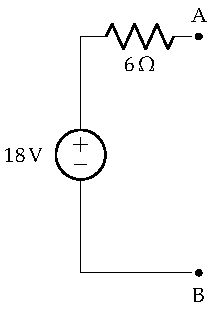
\includegraphics[scale=0.75]{figs/Conversion_Fuentes.pdf}
\hspace{1cm}
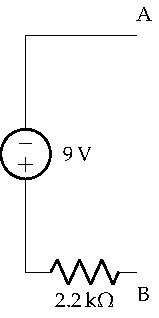
\includegraphics[scale=0.75]{figs/Conversion_Fuentes_2.pdf}
\hspace{1cm}
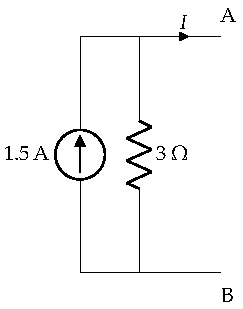
\includegraphics[scale=0.75]{figs/Conversion_Fuentes_3.pdf}
\hspace{1cm}
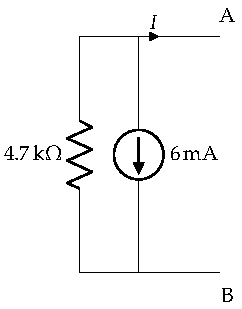
\includegraphics[scale=0.75]{figs/Conversion_Fuentes_4.pdf}

\section{}

\begin{minipage}{0.5\linewidth}
Calcula la resistencia equivalente entre A y B.
\end{minipage}
\begin{minipage}{0.5\linewidth}
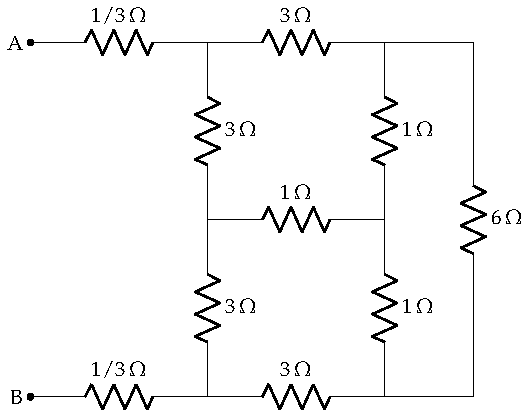
\includegraphics[scale=0.7]{figs/CircuitoResistivo_FM.pdf}
\end{minipage}

\section{}

Analiza el circuito de la figura mediante el método de las mallas, obteniendo:
\begin{enumerate}
\item Corriente de cada una de las ramas
\item Potencial en cada uno de los nudos, tomando como referencia el
  nudo A.
\end{enumerate}

Con estos resultados, realiza un balance de potencias comparando la potencia de los elementos activos y la de los elementos pasivos.

\begin{minipage}{0.4\linewidth}
  Datos:
  \begin{align*}
    R_1 = R_3 = R_6 &= \SI{3}{\ohm}\\
    R_2 = R_4 = R_5 &= \SI{2}{\ohm}\\
    \epsilon_1 &= \SI{245}{\volt}\\
    \epsilon_2 &= \SI{490}{\volt}\\
    \epsilon_3 &= \SI{735}{\volt}\\
  \end{align*}
\end{minipage}
\begin{minipage}{0.6\linewidth}
  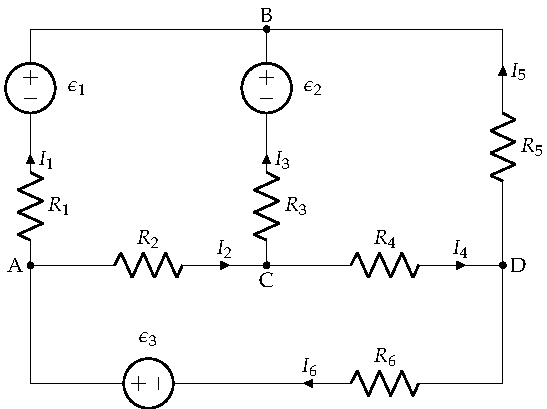
\includegraphics{figs/mallas1.pdf}
\end{minipage}

\section{}
Analiza el circuito de la figura mediante el método de las mallas, obteniendo la corriente de cada una de las ramas. Con este resultado calcula la diferencia de potencial entre A y B, y realiza un balance de potencias comparando la potencia de los elementos activos y la de los elementos pasivos.

\begin{minipage}{0.4\linewidth}
  Datos:
  \begin{align*}
    R_1 = R_2 &= \SI{1}{\ohm}\\
    R_3 &= \SI{2}{\ohm}\\
    R_4 &= \SI{3}{\ohm}\\
    R_5 &= \SI{4}{\ohm}\\
    \epsilon_1 &= \SI{118}{\volt}\\
    \epsilon_2 &= \SI{236}{\volt}\\
    \epsilon_3 &= \SI{118}{\volt}\\
  \end{align*}
\end{minipage}
\begin{minipage}{0.6\linewidth}
  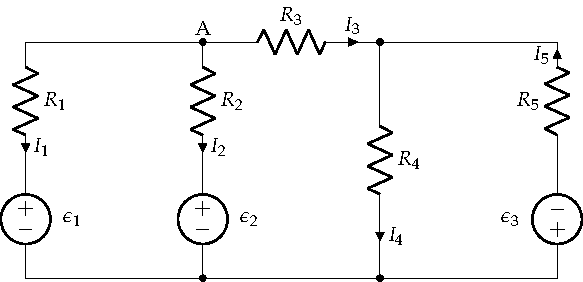
\includegraphics{figs/mallas2.pdf}
\end{minipage}


\clearpage

\section{}

En el circuito de la figura se debe emplear el método de los nudos para determinar:
\begin{itemize}
\item Las tensiones en los nudos A y B.
\item Las corrientes de todas las ramas.
\item El balance de potencias, diferenciando entre elementos activos y elementos pasivos.
\end{itemize}

\begin{minipage}[c]{0.3\linewidth}
  \begin{align*}
    \epsilon_1&=\SI{6}{\volt}\\
    \epsilon_2&=\SI{12}{\volt}\\
    \epsilon_3&=\SI{24}{\volt}\\
    I_{g1} &= \SI{15}{\ampere}\\
    I_{g2} &= \SI{9}{\ampere}\\
    I_{g3} &= \SI{6}{\ampere}\\
    R_{1}&= R_3 = R_4 = R_5 = \SI{2}{\ohm}\\
    R_{2}&= \SI{1}{\ohm}
  \end{align*}
\end{minipage}
\begin{minipage}[c]{0.7\linewidth}
  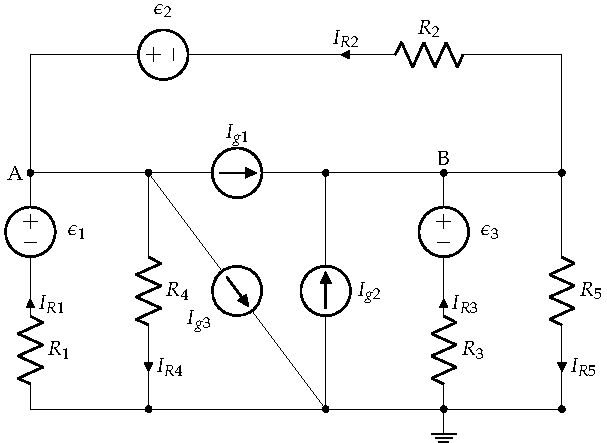
\includegraphics{figs/nudos_fuentes.pdf}
\end{minipage}

\subsection*{Solución}


Transformando las fuentes de tensión en fuentes de corriente obtenemos:

\[
\small{
\left(\begin{array}{ccc}
    1/R_1 + 1/R_2 + 1/R_4 & -1/R_2\\
    -1/R_2 & 1/R_2 + 1/R_3 + 1/R_5
  \end{array}\right) \cdot \left(\begin{array}{c}
    V_{A}\\
    V_{B}
  \end{array}\right) = 
\left(\begin{array}{c}
        E_1/R_1 + E_2/R_2 - I_1 - I_3\\
        -E_2/R_2 + I_1 + I_2 + E_3/R_3
      \end{array}\right)
  }
\]

La solución de esta ecuación matricial es $V_A = \SI{4}{\volt}$ y $V_B = \SI{14}{\volt}$. 

Con estos resultados podemos calcular las corrientes que circulan por las resistencias asociadas a los generadores de tensión:

\begin{align*}
V_A &= E_1 - I_{R1} R_1\\
V_{AB} &= E_2 - I_{R2} R_2\\
V_B &= E_3 - I_{R3} R_3\\
\end{align*}

\begin{align*}
I_{R1} &= \SI{1}{\ampere}\\
I_{R2} &= \SI{22}{\ampere}\\
I_{R3} &= \SI{5}{\ampere}
\end{align*}

Por tanto, los elementos activos aportan un total de \SI{642}{\watt}:

\begin{align*}
P_{I1} &= I_1 V_{BA} = \SI{150}{\watt}\\
P_{I2} &= I_2 V_{B} = \SI{126}{\watt}\\
P_{I1} &= I_3 (-V_{A}) = - \SI{24}{\watt}\\
P_{E1} &= E_1 I_{R1} = \SI{6}{\watt}\\
P_{E2} &= E_2 I_{R2} = \SI{264}{\watt}\\
P_{E3} &= E_3 I_{R3} = \SI{120}{\watt}
\end{align*}

Los elementos pasivos consumen un total de \SI{642}{\watt}:

\begin{align*}
P_{R1} &= I^2_{R1} R_1 = \SI{2}{\watt}\\
P_{R2} &= I^2_{R2} R_2 = \SI{484}{\watt}\\
P_{R3} &= I^2_{R3} R_3 = \SI{50}{\watt}\\
P_{R4} &= I^2_{R4} R_4 = \SI{8}{\watt}\\
P_{R5} &= I^2_{R5} R_5 = \SI{98}{\watt}
\end{align*}

\clearpage

\section{}
Aplica el método de los nudos en el circuito de la figura para determinar:
\begin{enumerate}
\item Los potenciales de los nudos A, B, C y D.
\item Las intensidades de corriente señaladas.
\item Carga, polaridad y energía almacenada en los condensadores,
  supuestos sin carga inicial.
\end{enumerate}

\begin{minipage}[c]{0.3\textwidth}
  \begin{align*}
    R_i &= \mathrm{i\ } \si{\ohm}\\
    C_i &= \mathrm{i\ } \si{\micro\farad}\\
    E_1 &= \SI{6}{\volt}\\
    E_2 &= \SI{18}{\volt}\\
    E_3 &= \SI{6}{\volt}\\
  \end{align*}
\end{minipage}
\begin{minipage}[c]{0.7\textwidth}
  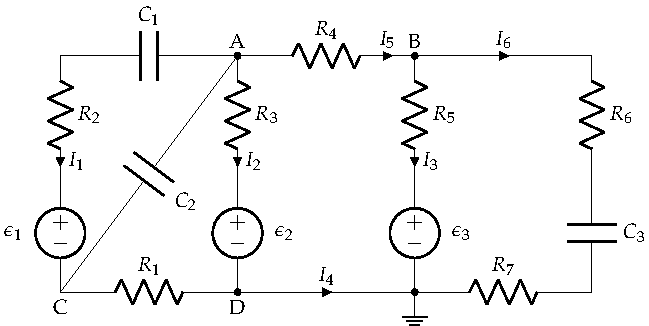
\includegraphics[width=\textwidth]{figs/nudos_condensadores.pdf}
\end{minipage}

\clearpage

\section{}

En el circuito de la figura debes determinar:
\begin{itemize}
\item Las intensidades señaladas.
\item Los potenciales en los puntos A, B, C, D, E y F.
\end{itemize}


\begin{minipage}[c]{0.2\linewidth}
  \begin{align*}
    \epsilon_{A}&=\SI{90}{\volt}\\
    \epsilon_{B}&=\SI{60}{\volt}\\
    \epsilon_{C}&=\SI{30}{\volt}\\
    R_{1}&= R_2 = R_3 = \SI{10}{\ohm}\\
    R_{4}&= R_5 = \SI{30}{\ohm}\\
    C_{1}&= \SI{10}{\micro\farad}\\
    C_{2}&= \SI{20}{\micro\farad}\\
    L_1 &= \SI{1}{\micro\henry}\\
    q^0_{C1} &= \SI{10}{\micro\coulomb}\\
    q^0_{C2} &= \SI{20}{\micro\coulomb}
  \end{align*}
\end{minipage}
\begin{minipage}[c]{0.8\linewidth}
  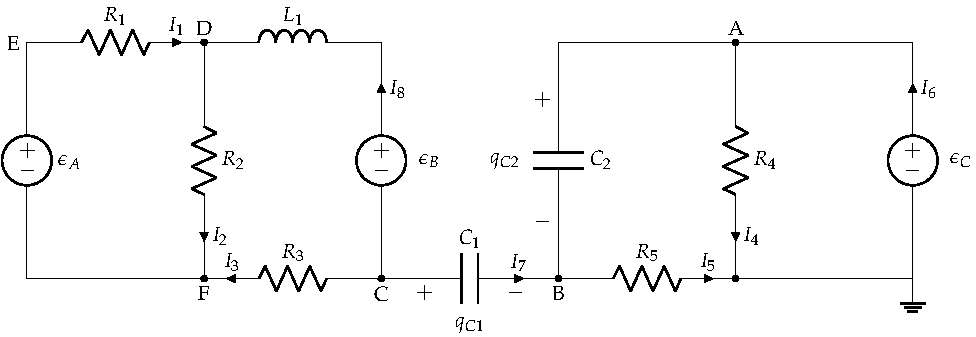
\includegraphics[scale = 0.8]{figs/mallas_carga_inicial.pdf}
\end{minipage}

\clearpage

\section{}

En el esquema de la figura los condensadores se conectaron sin
carga. Mediante el método de las mallas determina:
\begin{enumerate}
\item Intensidades de corriente señaladas.
\item Potenciales en los puntos A, B, C y D.
\item Polaridades, cargas, y energías de los condensadores.
\item Balance de potencias.
\end{enumerate}

\begin{minipage}[c]{0.3\linewidth}
  \begin{align*}
    \epsilon_{1}&=\SI{118}{\volt}\\
    \epsilon_{2}&=\SI{236}{\volt}\\
    \epsilon_{3}&=\SI{118}{\volt}\\
    R_{1}&= \SI{4}{\ohm}\\
    R_{2}&=R_{3}=\SI{1}{\ohm}\\
    R_{4}&= \SI{3}{\ohm}\\
    R_{5}&= \SI{2}{\ohm}\\
    C_{1}&=C_{2}=C_{3}=\SI{2}{\micro\farad}\\
    X_1 &= X_2 = X_3 = \SI{1}{\ohm}\\
  \end{align*}
\end{minipage}
\begin{minipage}[c]{0.7\linewidth}
  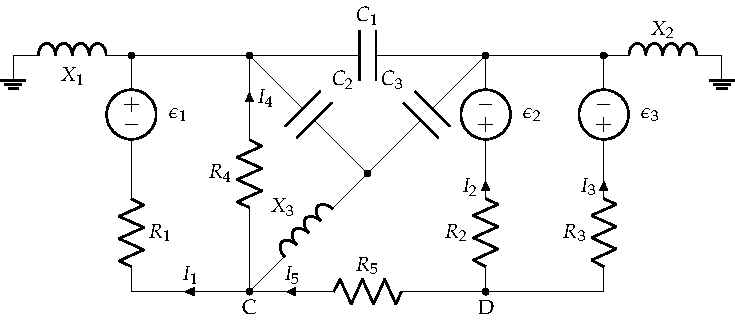
\includegraphics{figs/mallas_condensadores.pdf}
\end{minipage}

\subsection*{Solución}
Sustituimos los condensadores y las bobinas por sus equivalentes en un circuito de corriente continua. En el circuito resultante marcamos tres corrientes de malla dextrógiras, y planteamos la matriz correspondiente para resolver por mallas: 

\[
\small{
\left(\begin{array}{c}
    E_1\\
    E_2\\
    E_2 - E_3
  \end{array}\right) = \left(\begin{array}{ccc}
    R_1 + R_4 & -R_4 & 0\\
    -R_4 & R_4 + R_5 + R_2 & -R_{2}\\
    0 & -R_2 & R_2 + R_3
  \end{array}\right) \cdot \left(\begin{array}{c}
    I_{A}\\
    I_{B}\\
    I_{C}
  \end{array}\right)
}
\]

\[
\small{
\left(\begin{array}{c}
    118\\
    236\\
    118
  \end{array}\right) = \left(\begin{array}{ccc}
    7 & -3 & 0\\
    -3 & 6 & -1\\
    0 & -1 & 2
  \end{array}\right) \cdot \left(\begin{array}{c}
    I_{A}\\
    I_{B}\\
    I_{C}
  \end{array}\right)
}
\]

La solución es:

\begin{eqnarray*}
I_A & = & \SI{40}{\ampere}\\
I_B & = & \SI{54}{\ampere}\\
I_C & = & -\SI{32}{\ampere}
\end{eqnarray*}

Por tanto, las corrientes indicadas en el circuito son:

\begin{eqnarray*}
I_1 & = & \SI{40}{\ampere}\\
I_2 & = & \SI{-86}{\ampere}\\
I_3 & = &  \SI{32}{\ampere}\\
I_4 & = &  \SI{14}{\ampere}\\
I_5 & = &  \SI{54}{\ampere}
\end{eqnarray*}

Las tensiones en los puntos indicados son:

\begin{align*}
V_A &= \SI{0}{\volt}\\
V_B &= \SI{0}{\volt}\\
V_C &= I_4 \cdot R_4 = \SI{42}{\volt}\\
V_D &= I_5 \cdot R_5 + V_c = \SI{150}{\volt}\\
\end{align*}

Por tanto, las polaridades de los condensadores son las marcadas en la figura, con los valores de tensión siguientes:

\begin{eqnarray*}
U_{C1} = U_{BA} & = & \SI{0}{\volt}\\
q_1 = C_1 \cdot U_{C1} & = & \SI{0}{\micro\coulomb}\\
E_{C2} & = & \SI{0}{\joule}
\end{eqnarray*}

\begin{eqnarray*}
U_{C2} = U_{CA} & = & \SI{42}{\volt}\\
q_2 = C_2 \cdot U_{C2} & = & \SI{84}{\micro\coulomb}\\
E_{C2} & = & \SI{1.76}{\milli\joule}
\end{eqnarray*}

\begin{eqnarray*}
U_{C3} = U_{CB} & = & \SI{42}{\volt}\\
q_3 = C_3 \cdot U_{C3} & = & \SI{84}{\micro\coulomb}\\
E_{C3} & = & \SI{1.76}{\milli\joule}
\end{eqnarray*}

Finalmente, el balance de potencias calcula la potencia entregada por los elementos activos y la potencia consumida por los elementos pasivos.

La potencia total entregada por los elementos activos es $\SI{21240}{\watt}$:
\begin{eqnarray*}
P_{E1} = E_1 \cdot I_1 & = & \SI{4720}{\watt}\\
P_{E2} = E_2 \cdot (-I_2) & = & \SI{20296}{\watt}\\
P_{E3} = E_3 \cdot (-I_3) & = & \SI{-3776}{\watt}
\end{eqnarray*}

La potencia total consumida por los elementos pasivos también es $\SI{21240}{\watt}$:
\begin{eqnarray*}
P_{R1} = R_1 \cdot I_1^2 & = & \SI{6400}{\watt}\\
P_{R2} = R_2 \cdot I_2^2 & = & \SI{7396}{\watt}\\
P_{R3} = R_3 \cdot I_3^2 & = & \SI{1024}{\watt}\\
P_{R4} = R_4 \cdot I_4^2 & = & \SI{588}{\watt}\\
P_{R5} = R_5 \cdot I_5^2 & = & \SI{5832}{\watt}
\end{eqnarray*}

\clearpage

\section{}

En el circuito de la figura se debe determinar:
\begin{itemize}
\item Las corrientes señaladas.
\item El balance de potencias, diferenciando entre elementos activos y elementos pasivos.
\item Los potenciales en los puntos A, B y C.
\item La carga, polaridad y energía almacenada en los condensadores, supuestos sin carga inicial.
\end{itemize}

\begin{minipage}[c]{0.3\linewidth}
  \begin{align*}
    \epsilon_1&=\SI{1}{\volt}\\
    \epsilon_2&=\SI{7}{\volt}\\
    R_i &= \SI{1}{\ohm}\\
    C_i &= \SI{i}{\micro\farad}
  \end{align*}
\end{minipage}
\begin{minipage}[c]{0.7\linewidth}
  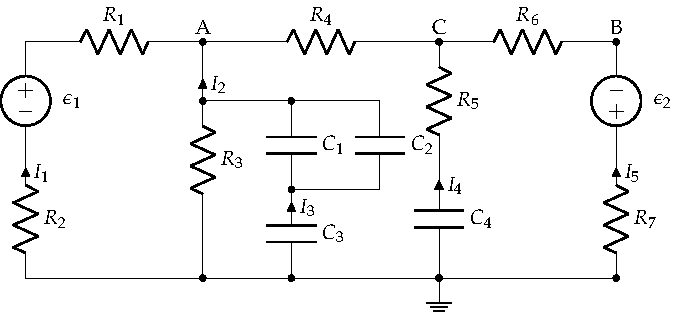
\includegraphics{figs/mallas_agrupacion_condensadores.pdf}
\end{minipage}

\clearpage

\section{}

El circuito de la figura está funcionando en regimen estacionario. Los condensadores estaban inicialmente descargados. Resuelve el circuito mediante el método que consideres conveniente para obtener los siguientes resultados:

\begin{enumerate}
\item Las intensidades señaladas.
\item Carga, polaridad y energía almacenada en los condensadores.
\item Balance de potencias.
\end{enumerate}


\begin{minipage}[c]{0.2\linewidth}
  Datos:
  \begin{align*}
    \epsilon_{1}&=\SI{40}{\volt}\\
    \epsilon_{2}&=\SI{22}{\volt}\\
    \epsilon_{3}&=\SI{20}{\volt}\\
    C_{1}&=C_{2}=C_{3}=\SI{2}{\micro\farad}\\
    R_{g1}&=R_{g2}=R_{g3}=\SI{4}{\ohm}\\
    R_{1}&=R_{2}=R_{3}=R_{4}=\SI{2}{\ohm}\\
    R_{5}&=R_{6}=R_{7}=\SI{1}{\ohm}
  \end{align*}
\end{minipage}
\begin{minipage}[c]{0.8\linewidth}
  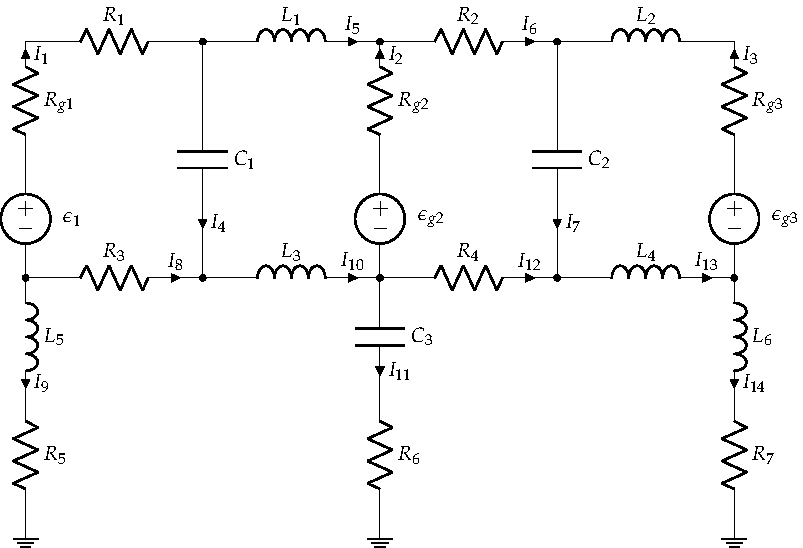
\includegraphics[scale = 0.8]{figs/mallas_condensadores_bobinas.pdf}
\end{minipage}

\subsection*{Solución}

Cuando el circuito se encuentra en régimen permanente, dado que las
fuentes son de corriente continua, los condensadores se sustituyen
por circuitos abiertos (inicialmente están descargados) y las bobinas
por cortocircuitos. De esta forma, el circuito original queda reducido
a tres mallas (A, B y C).

La resolución de este circuito mediante el método de las mallas se
sirve de la siguiente ecuación matricial:

\[
\left(\begin{array}{c}
E_{1}-E_{2}\\
E_{2}-E_{3}\\
0
\end{array}\right) = \left(\begin{array}{ccc}
R_{g1}+R_{1}+R_{g2}+R_{3} & -R_{g2} & -R_{3}\\
-R_{g2} & R_{g2}+R_{2}+R_{g3}+R_{4} & -R_{4}\\
-R_{3} & -R_{4} & R_{3}+R_{4}+R_{5}+R_{7}
\end{array}\right) \cdot \left(\begin{array}{c}
I_{A}\\
I_{B}\\
I_{C}
\end{array}\right)
\]
 y sustituyendo los valores de cada elemento:

\[
\left(\begin{array}{c}
18\\
2\\
0
\end{array}\right) = \left(\begin{array}{ccc}
12 & -4 & -2\\
-4 & 12 & -2\\
-2 & -2 & 6
\end{array}\right) \cdot \left(\begin{array}{c}
I_{A}\\
I_{B}\\
I_{C}
\end{array}\right)
\]
cuya solución es:

\begin{eqnarray*}
I_{A} & = & 2\, A\\
I_{B} & = & 1\, A\\
I_{C} & = & 1\, A
\end{eqnarray*}


Ahora debemos relacionar estas corrientes de malla con las corrientes
de rama señaladas en el circuito original (teniendo en cuenta que
las corrientes que circulan por ramas con condensadores son nulas):

\begin{eqnarray*}
I_{1} & = & I_{A}=2\, A\\
I_{2} & = & -I_{A}+I_{B}=-1\, A\\
I_{3} & = & -I_{B}=-1\, A\\
I_{4} & = & 0\, A\\
I_{5} & = & I_{A}=2\, A\\
I_{6} & = & I_{B}=1\, A\\
I_{7} & = & 0\, A\\
I_{8} & = & -I_{A}+I_{C}=-1\, A\\
I_{9} & = & -I_{C}=-1\, A\\
I_{10} & = & -I_{A}+I_{C}=-1\, A\\
I_{11} & = & 0\, A\\
I_{12} & = & -I_{B}+I_{C}=0\, A\\
I_{13} & = & -I_{B}+I_{C}=0\, A\\
I_{14} & = & I_{C}=1\, A
\end{eqnarray*}



\subsubsection*{Carga, polaridad y energía almacenada en los condensadores}


El condensador $C_{1}$ está conectado directamente a la rama compuesta
por la fuente $E_{2}$ y su resistencia $E_{g2}$ (debido a que la
bobina se comporta como un cortocircuito). Por tanto, suponiendo que
la polaridad positiva de este condensador corresponde a su borne superior,
la tensión de este condensador es:
\[
V_{C1}=E_{2}-I_{2}\cdot R_{g2}=22-(-1)\cdot4=26\, V
\]
siendo correcta la polaridad asignada por el signo positivo de este
resultado. La energía almacenada por el condensador es:
\[
E_{C1}=1/2\cdot V_{c1}^{2}\cdot C_{1}=0.676\, mJ
\]

El condensador $C_{2}$ está conectado directamente a la rama compuesta
por la fuente $E_{3}$ y su resistencia $E_{g3}$ (debido a que la
bobina se comporta como un cortocircuito). Por tanto, suponiendo que
la polaridad positiva de este condensador corresponde a su borne superior,
la tensión de este condensador es:
\[
V_{C2}=E_{3}-I_{3}\cdot R_{g3}=20-(-1)\cdot4=24\, V
\]
siendo correcta la polaridad asignada por el signo positivo de este
resultado. La energía almacenada por el condensador es:
\[
E_{C2}=1/2\cdot V_{c2}^{2}\cdot C_{2}=0.576\, mJ
\]


El condensador $C_{3}$ está en paralelo con la resistencia $R_{4}$
y la resistencia $R_{7}$ (debido a que las bobinas se comportan como
un cortocircuito y a que por la resistencia $R_{6}$ no circula corriente).
Por tanto, suponiendo que la polaridad positiva de este condensador
corresponde a su borne superior, la tensión de este condensador es:
\[
V_{C3}=I_{12}\cdot R_{4}+I_{14}\cdot R_{7}=0+1\cdot1=1\, V
\]
siendo correcta la polaridad asignada por el signo positivo de este
resultado. La energía almacenada por el condensador es:
\[
E_{C3}=1/2\cdot V_{c3}^{2}\cdot C_{3}=1\,\mu J
\]



\subsubsection*{Balance de potencias}


\begin{eqnarray*}
P_{E1} & = & E_{1}\cdot I_{1}=80\, W\\
P_{E2} & = & E_{2}\cdot I_{2}=-22\, W\\
P_{E3} & = & E_{3}\cdot I_{3}=-20\, W\\
P_{T} & = & P_{E1}+P_{E2}+P_{E3}=38\, W
\end{eqnarray*}


\begin{eqnarray*}
P_{Rg1} & = & I_{1}^{2}\cdot R_{g1}=16\, W\\
P_{Rg2} & = & I_{2}^{2}\cdot R_{g2}=4\, W\\
P_{Rg3} & = & I_{3}^{2}\cdot R_{g3}=4\, W\\
P_{R1} & = & I_{1}^{2}\cdot R_{1}=8\, W\\
P_{R2} & = & I_{6}^{2}\cdot R_{2}=2\, W\\
P_{R3} & = & I_{8}^{2}\cdot R_{3}=2\, W\\
P_{R4} & = & I_{12}^{2}\cdot R_{4}=0\, W\\
P_{R5} & = & I_{9}^{2}\cdot R_{5}=1\, W\\
P_{R6} & = & 0\, W\\
P_{R7} & = & I_{14}^{2}\cdot R_{7}=1\, W
\end{eqnarray*}
siendo que la suma de estas potencias individuales coincide con la
potencia total activa.

\end{document}





